\documentclass{article}
\usepackage{hyperref}
\usepackage{lscape}
\usepackage{graphicx}
\hypersetup{
    colorlinks=true,
    linkcolor=blue,
    filecolor=magenta,
    urlcolor=cyan,
}
% Default fixed font does not support bold face
\DeclareFixedFont{\ttb}{T1}{txtt}{bx}{n}{10} % for bold
\DeclareFixedFont{\ttm}{T1}{txtt}{m}{n}{10}  % for normal

% Custom colors
\usepackage{color}
\definecolor{deepblue}{rgb}{0,0,0.5}
\definecolor{deepred}{rgb}{0.6,0,0}
\definecolor{deepgreen}{rgb}{0,0.5,0}

\usepackage{listings}

% Python style for highlighting
\newcommand\pythonstyle{\lstset{
language=Python,
basicstyle=\ttm,
otherkeywords={self},             % Add keywords here
keywordstyle=\ttb\color{deepblue},
emph={MyClass,__init__},          % Custom highlighting
emphstyle=\ttb\color{deepred},    % Custom highlighting style
stringstyle=\color{deepgreen},
frame=tb,                         % Any extra options here
showstringspaces=false            %
}}


% Python environment
\lstnewenvironment{python}[1][]
{
\pythonstyle
\lstset{#1}
}
{}

% Python for external files
\newcommand\pythonexternal[2][]{{
\pythonstyle
\lstinputlisting[#1]{#2}}}

% Python for inline
\newcommand\pythoninline[1]{{\pythonstyle\lstinline!#1!}}
\title{ECE 590.14 \protect\\ Midterm Report \protect\\ Explorative text analysis of song lyrics using topic modelling.}
\author{Kedar Prabhudesai}
\date{\today}
\begin{document}
\maketitle
  \section{Introduction}
  In this project, I have attempted to perform some explorative analysis of song lyrics data using topic modelling. Topic models use an unsupervised learning approach, i.e. they do not require manually labelled training data, and categorize commonly co-uccurring words into similar topics. Given the success of topic modelling for categorizing documents, this analysis could potentially help in classifying songs based on their lyrical content.
  \section{Workflow}
  The general workflow of the key steps involved in this project is shown in \href{fig:flow}{Figure 1}. Broadly speaking the steps can be categorized into two main stages viz. data acquistion and data analysis.
    \subsection{Data acquisition}
    Initially I attempted to scrap lyrics data from \href{http://azlyrics.com}{www.azlyrics.com}. I was able to extract lyrics for a few songs, but later the website stopped responding. Figuring out why I couldn't extract data from the website turned out to be challenging, and probably the most time I spent during this project. After some online research particularly on  \href{https://www.scrapehero.com/how-to-prevent-getting-blacklisted-while-scraping/}{this} website, I learnt that since I was making too many read requests per second, my IP address was probably blocked. Learning from my earlier mistake, I decided to write a new web scraper for extracting lyrics from \href{http://lyricsfreak.com}{www.lyricsfreak.com}. This time I ensured that my read requests were spaced out, allowing around 15 seconds betwen every read request. Next, some details regarding the acquired data is provided. The following artists/bands ($n = 15$) were chosen to extract lyrics:
    \begin{itemize}
        \item Adele
        \item Ariana Grande
        \item Beatles
        \item Beyonc\'e Knowles
        \item Bruno Mars
        \item Coldplay
        \item Ed Sheeran
        \item Ellie Goulding
        \item John Legend
        \item Justin Bieber
        \item Justin Timberlake
        \item Miley Cyrus
        \item Rihanna
        \item Selena Gomez
        \item Taylor Swift
    \end{itemize}
    This is a summary of the web scraping operation. The following Python packages were used to perform these operations: \pythoninline{nltk, BeautifulSoup, urllib} and \pythoninline{re}\\
    \underline{\emph{Step 1}}: The webpage associated with each artist was analysed. This webpage consisted of links to other webpages which contained song lyrics. Since the page consisted of other unwanted links too, links related to lyrics only were identified by using a simple \pythoninline{regexp} search operation. This way, links for first $60$ song lyrics for each artist were selected.\\
    \underline{\emph{Step 2}}: Using the links from the previous step, `html' data at each link was extracted and filtered to retain only lyrical data. In this manner, lyrics from $871$ songs were extracted. Since some links did not contain any lyrical information, the total number of songs was less than $900$ ($15 \times 60$).\\
    \underline{\emph{Step 3}}: After extracting the lyrics, they we cleaned up to remove punctuations, unnecessary unicode symbols and stop words.

    \subsection{Data analysis using topic model}
    \underline{\emph{Step 1}}: Before running a topic model, each document i.e. lyrics for each song, was represented as bag-of-words (BoW). To get the BoW representation of each document, first the vocabulary i.e. a list of non-repeating (unique) words present in the entire corpus was determined. The total number of unique words ended up being $~8700$. Next, the number of instances of each word in the vocabulary per document was determined, which gives the bag-of-words representation for each document.\\
    \underline{\emph{Step 2}}: I used the latent Dirichlet allocation (LDA) topic model \cite{blei}  which is one of the most popular topic models used for discovering topics from text data. The LDA topic model infers the following latent structure from data:
    \begin{itemize}
      \item Topics, which are distributions over the vocabulary in the corpus.
      \item Per document mixing proportions of topics.
      \item Per word topic assignment.
    \end{itemize}
    I used Markov chain Monte Carlo Gibbs sampling \cite{geman} algorithm to infer the latent structure from data. Matlab implementation of the same provided by \cite{griffiths} was used in the analysis. For this analysis, I set the number of topics, $K=20$. The hyperparameters for the priors in the model were chosen as a function of the number of topics.

  \section{Results}
  \href{fig:t1Fig}{Figure 2} and \href{fig:t2Fig}{Figure 3} show the extracted topics after running the LDA topic model. The ordering of the words is sorted in desceding order and the top $20$ words in each topic are displayed. We can see from the results that the topic model does a decent job of grouping words belonging to similar topics with the following examples:
  \begin{itemize}
    \item Topic 2 seems to be related to \emph{`love'}, with words like ``love, kiss, forever, remember, never, eyes, mind, promise, lips".
    \item Topic 3 seems to be related to \emph{`infatuation'}, with words like ``girl, crazy, touch, whoa, damn, hot".
    \item Topic 6 seems to have \emph{`artist'} related words like ``bieber, beyonc\'e".
    \item Topic 7 seems to be related to \emph{`break-up'}, with words like ``can't, come, back, life, stop, please, miss, waiting, running, holding".
    \item Topic 11 seems to be related to \emph{`sadness'}, with words like ``dont, cry, mean, falling".
    \item Topic 14 seems to be related to \emph{`partying'}, with words like ``tonight, hands, babe, music, party, play, put, lover".
  \end{itemize}
  Having said that, there are also some topics which have words which cannot be related to each other, like the following:
  \begin{itemize}
    \item Topic 16 has words like ``bad, need, good, christmas, floor, blood, wave".
    \item Topic 9 has words like ``yeah, hard, two, die, yes, take, days".
  \end{itemize}
  \section{Discussion}
  As I was analysing these results, I realized how hard a problem this is. Songs convey very complex set of emotions with commonly used everyday words. Earlier applications of topic models like scientific documents exploit the fact that specific scientific disciplines have very well defined set of words that co-occur between documents within a discipline. On the contrary, song lyrics have a lot of words which can be common between topics. For example, words like `life', `cry' can occur simultaneously in several topics.
  \section{Future Work}
  There are several avenues which can be explored to take this research forward. Some of which are discussed here:
  \begin{itemize}
    \item \underline{\emph{Vary topic model parameters}}: It is well known in topic modelling literature that results of topic models are very sensitive to model parameters viz. number of topics and prior hyperparameters. It would be interesting to see how topics change with these parameters.
    \item \underline{\emph{Analyse lyrics in a particular genre}}: I was probably too ambitious with this project to include artists and bands from a variety of genres. I would hypothesize that topics may be more closely related to songs belonging to the same genre. For example, country music may be more topics associated with `America' and/or patriotism.
    \item \underline{\emph{Augmenting non text data}}: It would be interesting to see what would happen if the sound data from the actual music files can be incorporated in the analysis along with song lyrics data.
  \end{itemize}
  \section{Figures}
    \begin{figure}
      \begin{center}
      
\includegraphics[width=5cm]{Flowchart.png}
      \end{center}
      \caption{Flowchart of various steps involved}
      \label{fig:flow}
    \end{figure}\\
    \begin{figure}
      \begin{center}
      
\includegraphics[width=15cm]{LDAGraphicalModel.png}
      \end{center}
      \caption{Latent Dirichlet Allocation}
      \label{fig:lda}
    \end{figure}
    \begin{landscape}
      \begin{figure}
        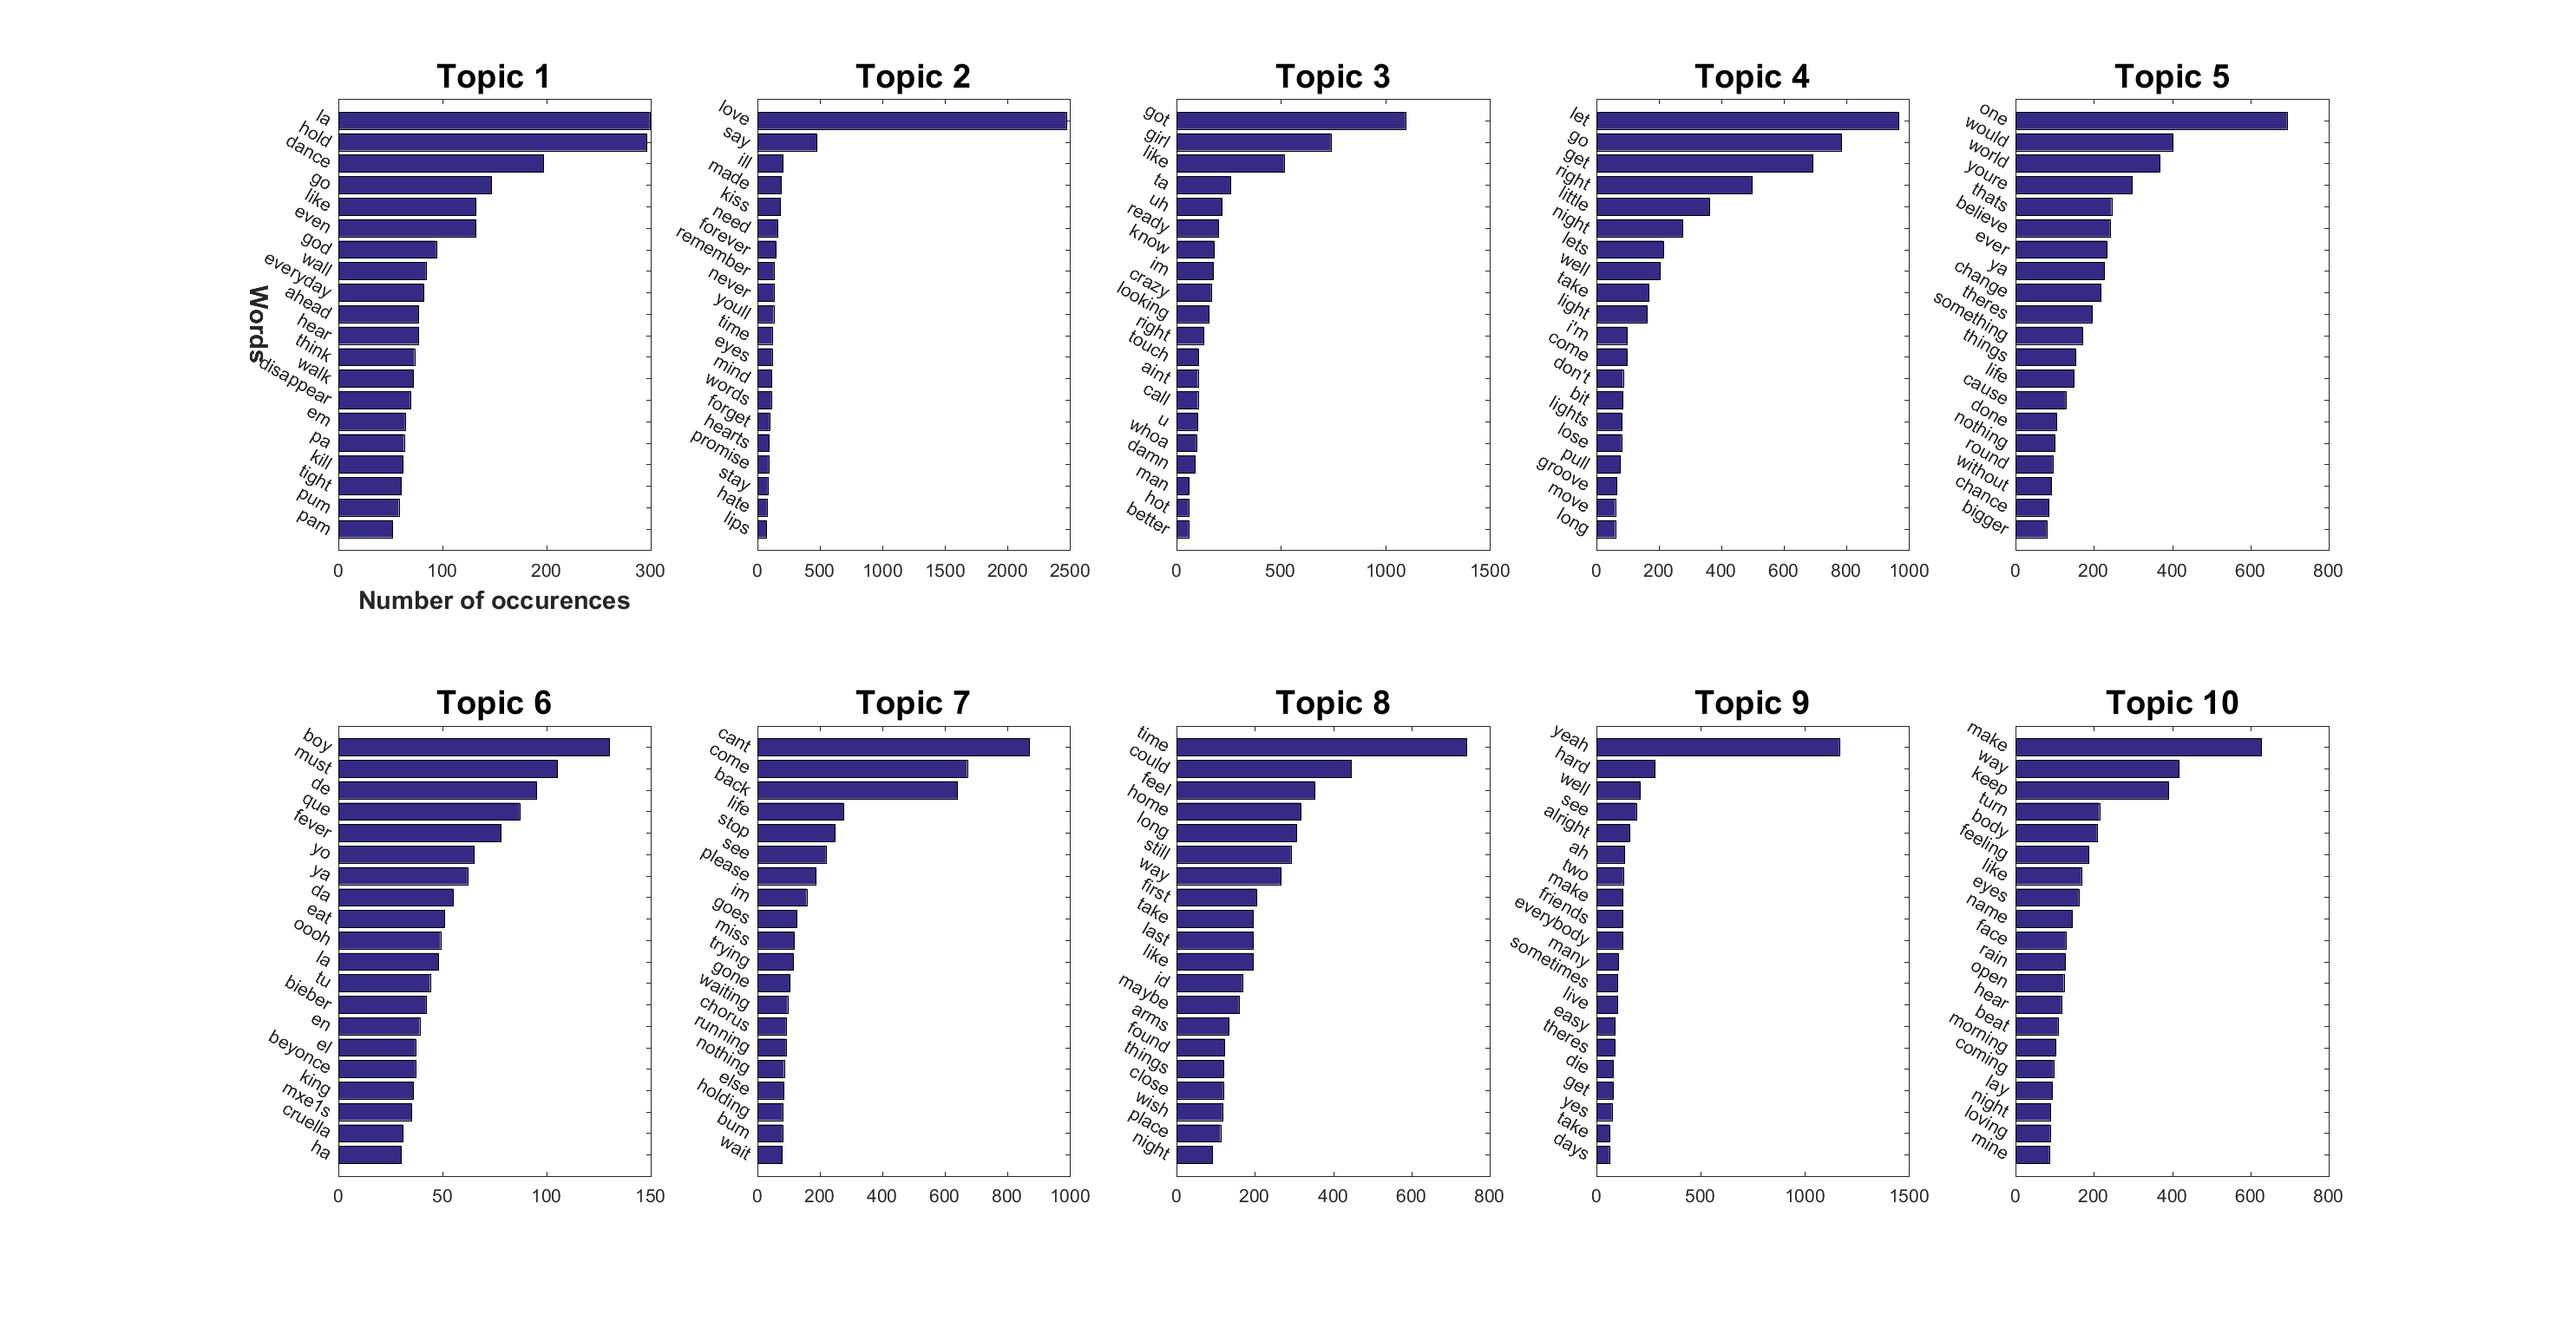
\includegraphics[width=\linewidth]{AllTopics_1.png}
        \caption{Topics 1 through 10}
        \label{fig:t1Fig}
      \end{figure}
    \end{landscape}
    \begin{landscape}
      \begin{figure}
        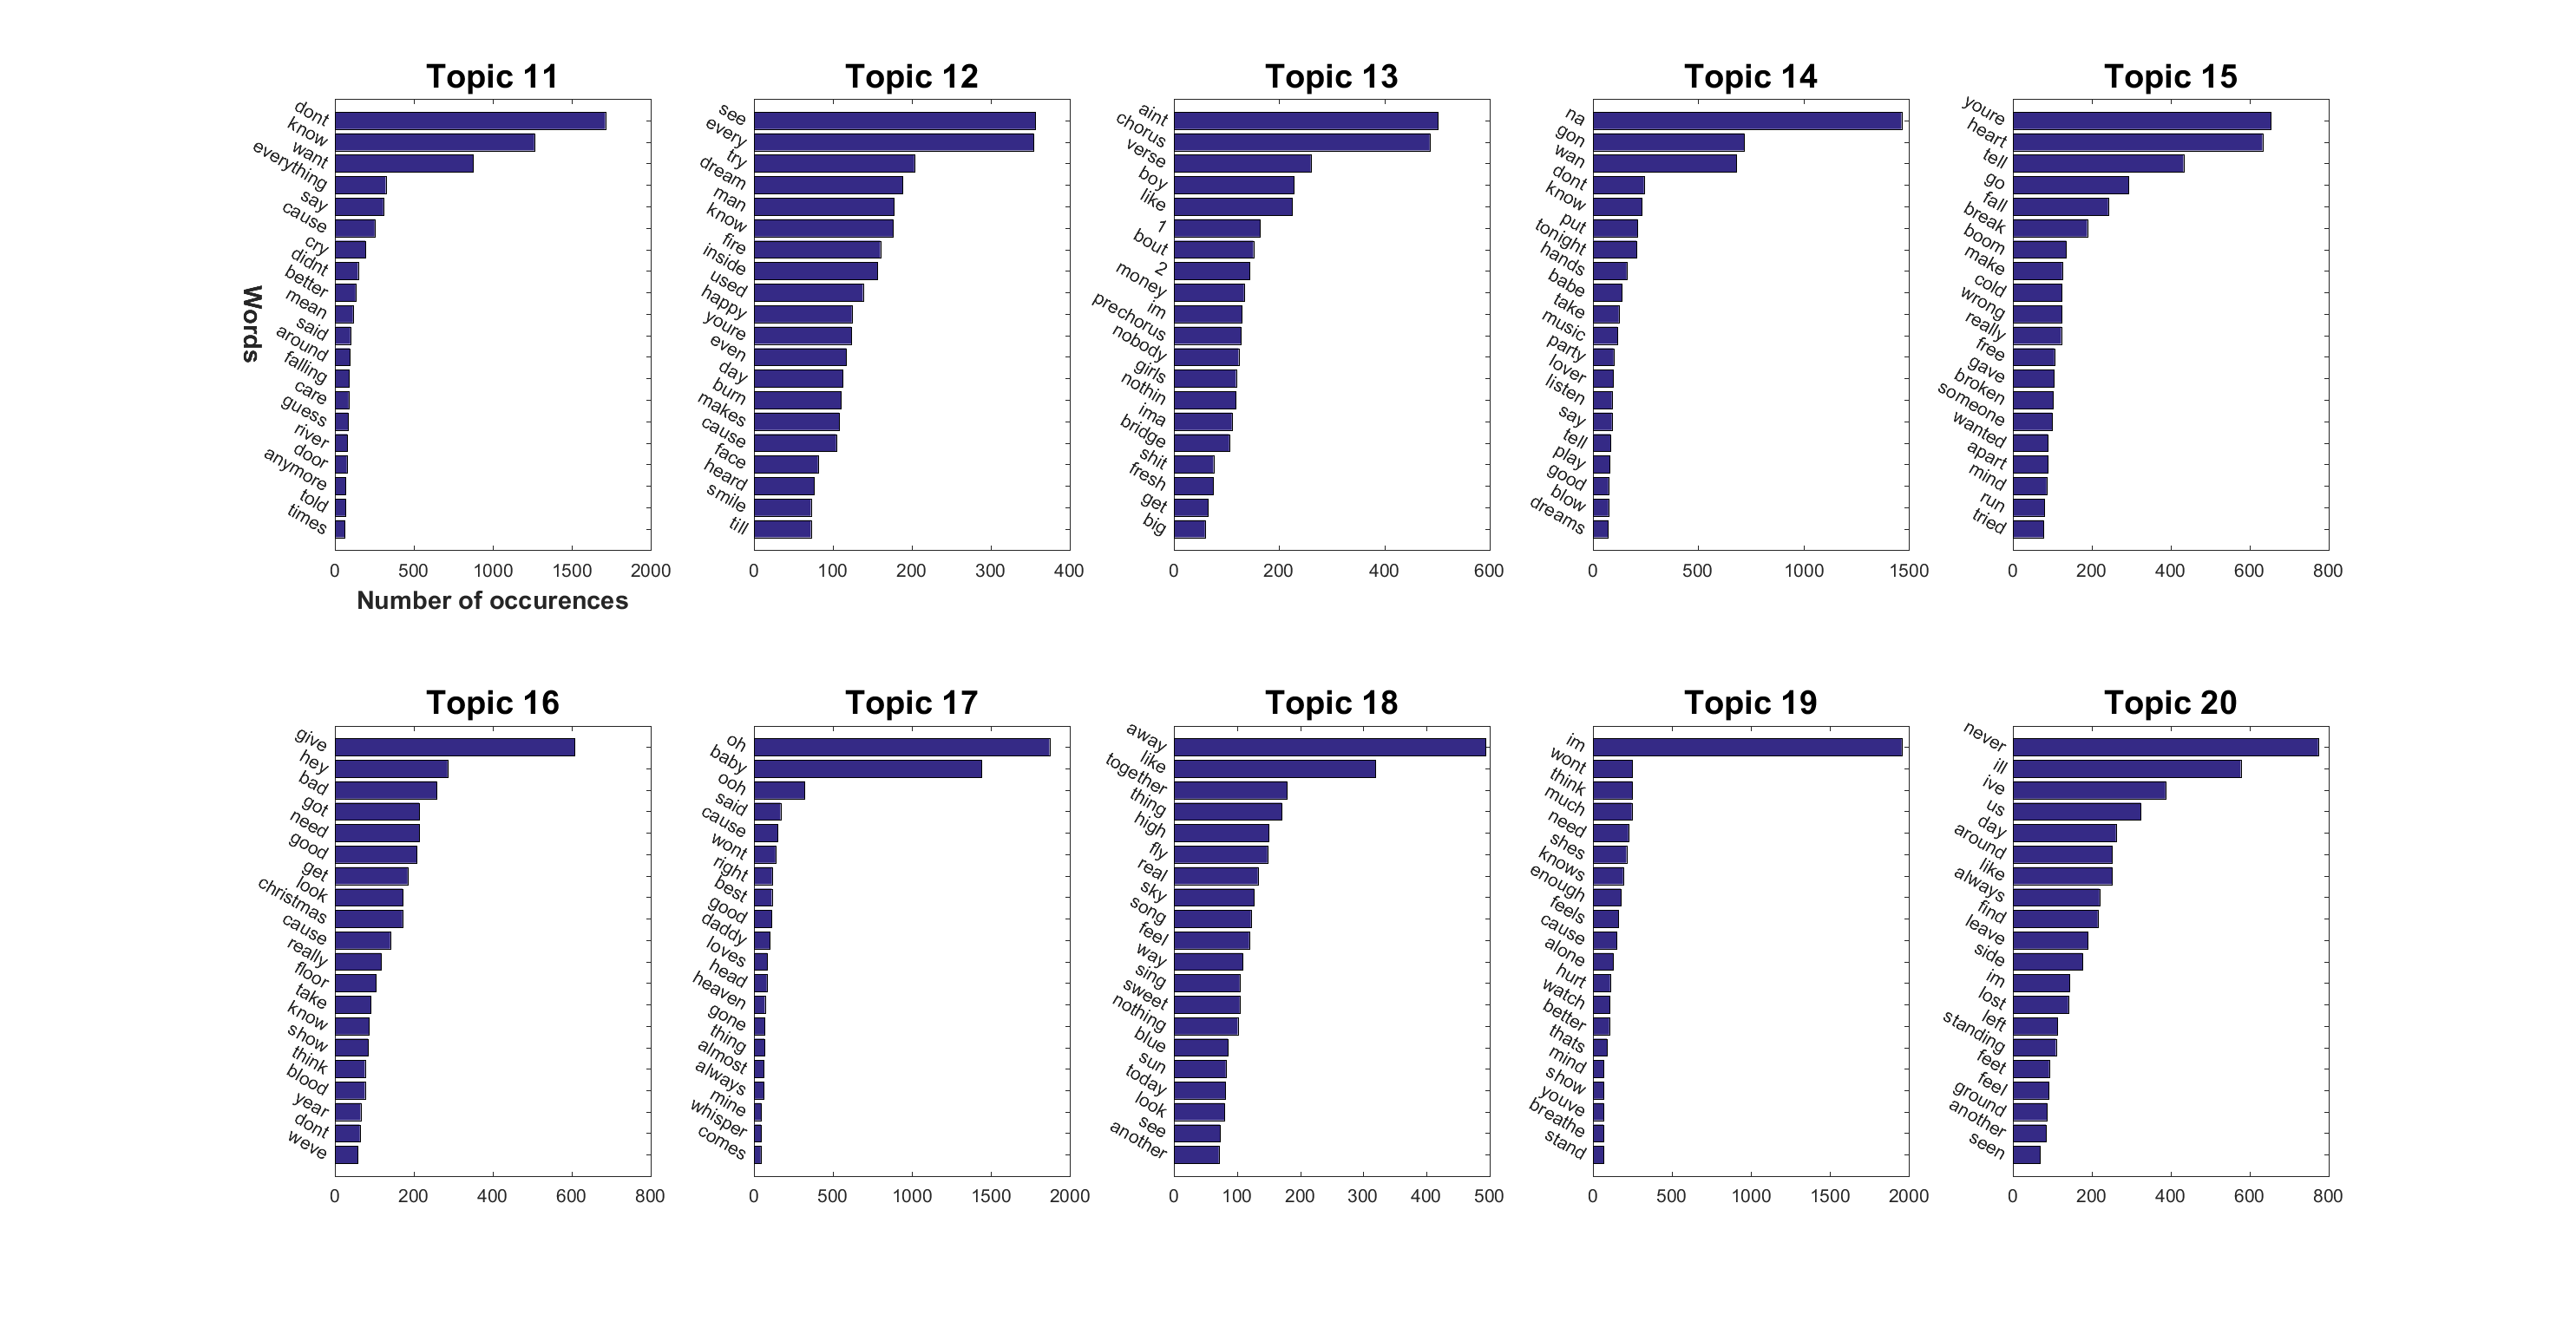
\includegraphics[width=\linewidth]{AllTopics_2.png}
        \caption{Topics 11 through 20}
        \label{fig:t2Fig}
      \end{figure}
    \end{landscape}

  \begin{thebibliography}{9}
    \bibitem{blei}
    Blei, David M., Andrew Y. Ng, and Michael I. Jordan. "Latent dirichlet allocation." \emph{Journal of machine Learning research} 3.Jan (2003): 993-1022.
    \bibitem{geman}
    Geman, Stuart, and Donald Geman. "Stochastic relaxation, Gibbs distributions, and the Bayesian restoration of images." \emph{IEEE Transactions on pattern analysis and machine intelligence} 6 (1984): 721-741.
    \bibitem{griffiths}
    Griffiths, Thomas L., and Mark Steyvers. "Finding scientific topics." \emph{Proceedings of the National academy of Sciences} 101.suppl 1 (2004): 5228-5235.
  \end{thebibliography}
\end{document}
